\chapter{软件补丁兼容性检测方法}
\section{兼容性问题}
\label {sec_problem}
如前所述,随着软件版本的演进,往往会发生专为某版本设计的补丁无法适用于新版本代码的情况。实际上也就是软件补丁在应用到新版本时出现了兼容性问题,而如果要为新版本代码重新开发适用的补丁,又会耗时耗力极大。由于在实际开发过程中,这一问题普遍存在而且较为复杂。因此,本文将尝试去解决这样一个软件补丁在不同版本间共享的问题。

考虑前文中提到的应用场景:
\begin{itemize}
	\item 某项目团队在开发过程中使用了某开源第三方软件,并针对该开源软件开发了专门的补丁以适用于本项目。
	\item 当第三方软件更新到新版本,在集成该新版本的时候,想知道原补丁是否还能继续使用。
\end{itemize}

为了解决这样一个补丁兼容性检测的问题,首先我们需要知道补丁在应用时可能会出现什么问题。如果按照出现的错误类型来划分,则在其他版本代码上应用该补丁可能会导致两类错误。

首先,在应用补丁时,补丁中引入的变更可能会破坏代码中原有的语法结构,从而出现语法错误。该类错误使用编译器即可发现,且容易解决。例如,当补丁所要删除的代码行已经不在原位置时,此时应用补丁会导致程序中错误的代码行被删除,原来的合法语法结构因此被破坏。

其次,在应用补丁时,补丁中的变更会对其他语法结构产生语义上的影响,从而导致程序行为发生变化。例如,某条变更可能会修改对某个变量的赋值,那么在其之后引用该变量的某条件语句的执行就会受到该变更的影响。当补丁应用于其所适用的代码版本时,这种语义变化是可控的,然而当补丁应用于其他版本的代码时,这种语义变化就可能是开发该版本代码的工程师所无法预知的。也就是说,此时补丁中的变更可能会引发语义层面的错误,导致程序的功能正确性受到影响。

显然,语法错误是易发现、好解决的,直接使用编译器就可得到相应的错误提示。而对于语义变化所导致的功能性错误来讲,这类错误则是难以发现的,我们很难直接发现某条变更会影响到程序中的某个语法结构,从而导致其功能正确性受到影响。

因此,在解决补丁兼容性问题的时候,本文将着重去解决语义上的兼容性问题。

事实上,考虑到版本更新也可以使用补丁来完成,那么在上文的应用场景中,该问题就可以从另一种角度来看待。如果将第三方软件的升级过程以打补丁的方式实现,那么在在集成该新版本的时候,原补丁是否能够继续使用的问题就可以转化为原补丁是否会和升级补丁产生冲突的问题。也就是说,软件补丁对于其他版本的适用性可以从补丁之间的冲突这一角度来考虑。

由于每个补丁都可以视作一系列的变更集合,其中的每条变更都会修改原有代码版本的语法结构,并可能会对其他语法结构造成语义上的影响,那么从这一角度来看时,补丁兼容性问题就得到了简化。我们可以找到每个补丁中的变更所影响到的程序语法结构的集合,并探讨这两个集合之间是否存在一定的交集,显然,如果两个补丁中的变更影响到了相同的语法结构,那么该受影响的代码位置就是可能出现冲突的。

这是由于该位置上的语法结构受到了双重影响,然而这些影响之间可能是有冲突的,无法共存的。例如对某条件判断语句来说,原补丁在某处对其引用的变量值进行了修改,使得条件语句中该值增加,而升级补丁中在另外一处对该变量的修改则会导致条件语句中其值减少,显然,这样的双重影响是矛盾的。

当然,在某些情况下,这样的双重影响也是可以共存的。例如上文条件判断语句的例子中,如果两个补丁中的修改都会导致该条件语句中引用的某变量值增加,那么这样的双重影响就可能是兼容的。

因此,这种双重影响的情况是否会导致冲突需要人工分析来辅助判断。

可见,软件补丁的兼容性检测问题实际上可以归结为多次变更之间的冲突检测。由于语法错误易于察觉,本文以后所提及的冲突检测都将只针对语义冲突进行检测。

\section{检测方法概述}
\label {sec_method}

根据前一节中的问题介绍,我们可以发现,该兼容性问题的解决过程可以分为三步。首先,我们需要将软件补丁应用于其他版本的代码上,并防止该过程中引入语法错误。其次,我们需要找到补丁中的变更所影响到的其他语法结构,也就是后文中所提出的变更影响域的概念。最后,我们根据找到的变更影响域,进行冲突检测。

因此,本文中提出了一种软件补丁兼容性的检测方法,该方法的整体流程可以参考图\ref {all_flow}。该检测方法的输入包括$v_1$版本和$v_2$版本的代码,以及适用于$v_1$版本的补丁p。其中版本$v_1$为旧版本,版本$v_2$为新版本。

\begin{figure}[H]
	\centering
	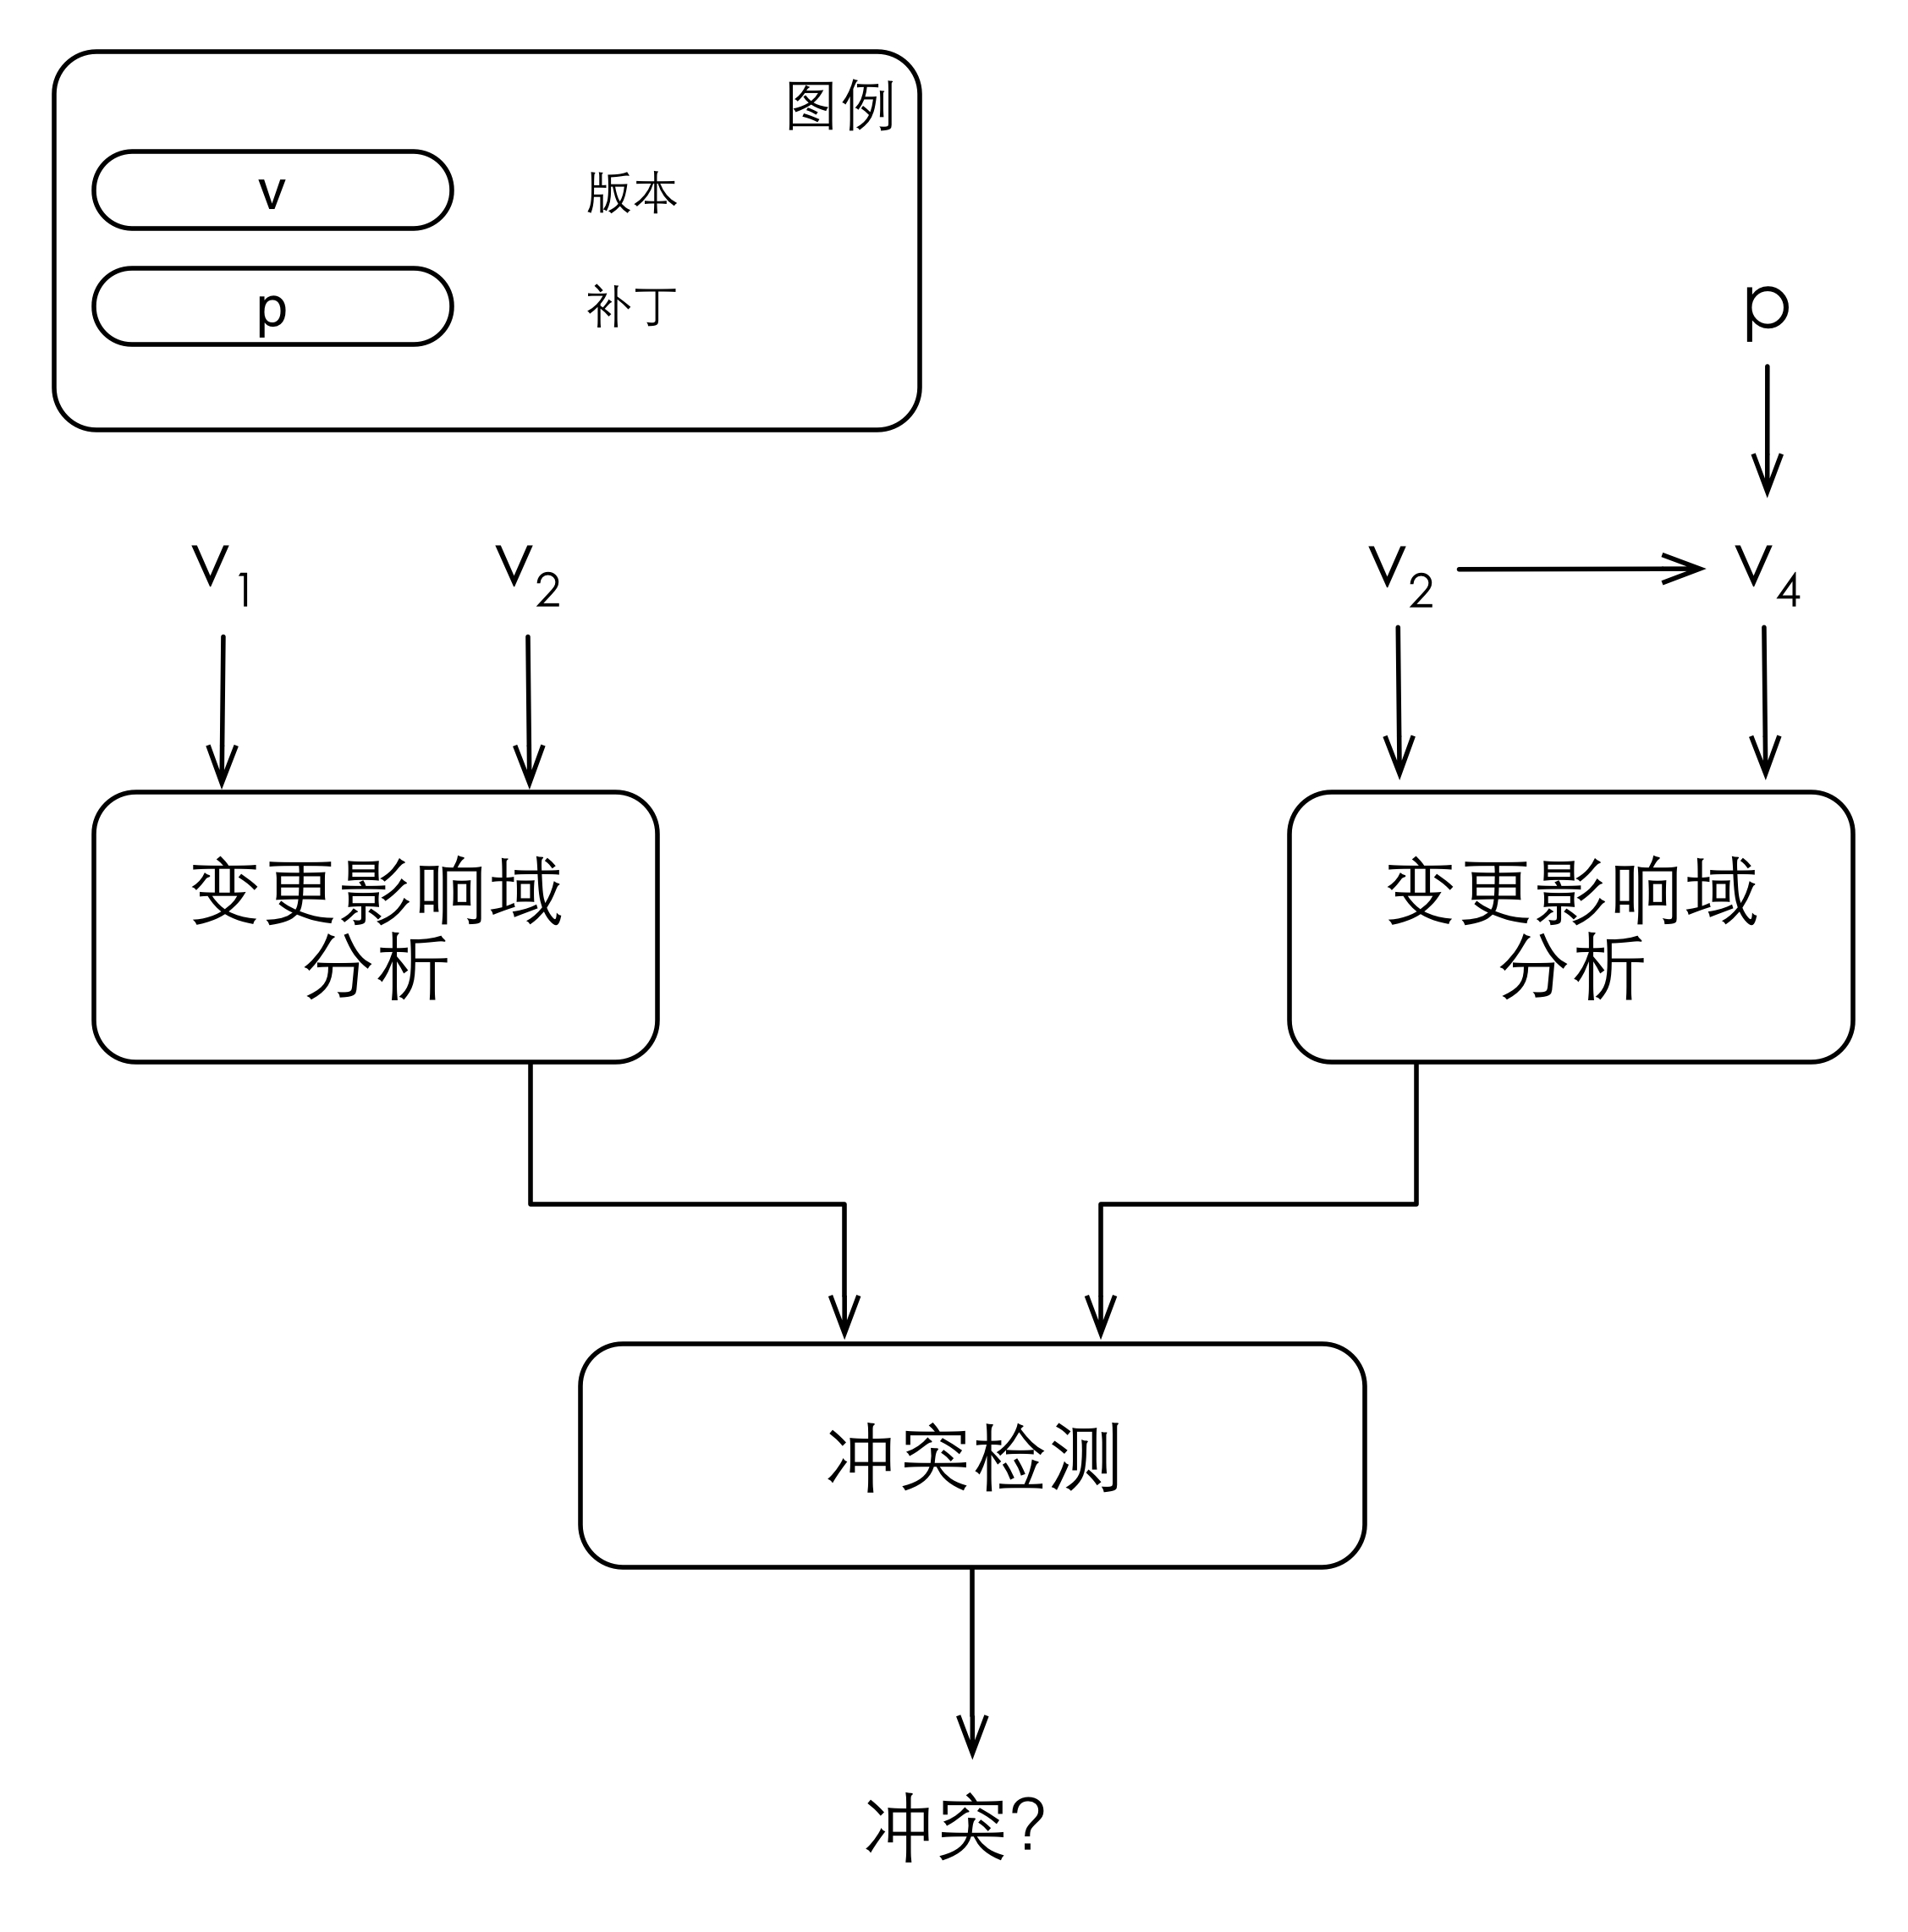
\includegraphics[height=.6\columnwidth]{chap03_all_now}
	\caption {解决方案}
	\label {all_flow}	
\end{figure}

该方法可以检测版本$v_1$到版本$v_2$的升级过程中所引入的变更是否会与补丁p在版本$v_2$中所引入的变更发生冲突。之所以选择以版本$v_2$作为基准来进行冲突检测,是由于在实际过程中,应用该检测方法之前还需要将补丁p应用至代码版本$v_2$,以便完成补丁应用的过程。

本文采用了版本合并的方法来解决该过程中可能引入的语法错误,其流程可以简述如下:
\begin{enumerate}
	\item 将补丁p应用到版本$v_1$,获得旧版本应用补丁后的代码,其版本为$v_3$。
	\item 采用三路归并算法将版本$v_2$和$v_3$进行合并,获得新版本应用补丁后的代码,其版本为$v_4$。
	\item 解决分支合并中可能出现的冲突问题。
\end{enumerate}

最后所得到的$v_4$版本代码即为我们所需要的在版本$v_2$上应用了补丁p中变更的新版本代码。

由于该合并过程较为简单,可以直接使用git等版本控制系统完成,以后的章节中将不再赘述,只在实验部分给出该过程相应的结果与分析。本文在以后的章节中将直接考虑对从版本$v_1$到$v_2$的升级过程中引入的变更与从版本$v_2$到$v_4$的升级过程中引入的变更进行冲突检测。

下面对该检测方法中所涉及到的过程进行概述。

首先,该检测方法中提出了一种软件变更影响域分析方法,该分析方法能够找到不同版本的代码间的变更集合,并以此为依据进行分析,最后找到变更集合所对应的语义影响域,即变更影响域,该变更影响域中包含了所有受到变更集合影响的程序语法结构。具体的变更影响域分析过程和变更影响域等相关概念的定义可以参考章节\ref {chap_impact}中的叙述。

其次,该检测方法根据得到的不同变更影响域,使用软件变更冲突检测方法判定这些变更影响域之间是否存在着语义上的冲突。该软件变更冲突检测方法的相关实现和定义可以参考章节\ref {chap_conflict}中的叙述。

本文根据此处提出的兼容性检测方法进行了相应的工具实现。按照兼容性检测方法的流程,该检测工具可以划分为两个模块:
\begin{itemize}
	\item 影响域分析模块:实现解决方案中的软件变更影响域分析过程。
	\item 冲突判定模块:实现解决方案中的软件变更冲突检测方法。
\end{itemize}

这些模块的实现过程可以分别参考相关章节中的叙述。

\section{本章小结}
本章中主要介绍了软件补丁兼容性问题和其检测方法的概述。
章节\ref {sec_problem}中介绍了补丁兼容性问题和其缘由。
章节\ref {sec_method}中对补丁兼容性检测方法和其工具实现进行了简要介绍。详细的介绍参见后续章节。


